%%%%%%%%%%%%%%%%%%%%%%%%%%%%%%%%%%%%%%%%%%%%%%%%%%%%%%%
%% Bachelor's & Master's Thesis Template             %%
%% Copyleft by Artur M. Brodzki & Piotr Woźniak      %%
%% Faculty of Electronics and Information Technology %%
%% Warsaw University of Technology, 2019-2020        %%
%%%%%%%%%%%%%%%%%%%%%%%%%%%%%%%%%%%%%%%%%%%%%%%%%%%%%%%

\documentclass[
    left=2.5cm,         % Sadly, generic margin parameter
    right=2.5cm,        % doesnt't work, as it is
    top=2.5cm,          % superseded by more specific
    bottom=3cm,         % left...bottom parameters.
    bindingoffset=6mm,  % Optional binding offset.
    nohyphenation=false % You may turn off hyphenation, if don't like.
]{eiti/eiti-thesis}

\langpol % Dla języka angielskiego mamy \langeng
\graphicspath{{img/}}             % Katalog z obrazkami.
\addbibresource{bibliografia.bib} % Plik .bib z bibliografią

\begin{document}

%--------------------------------------
% Strona tytułowa
%--------------------------------------
\MasterThesis % Dla pracy inżynierskiej mamy \EngineerThesis
\instytut{Infrastruktury,
Transportu i Mobilności}
\kierunek{E-biznes}
\title{
Czy kierownik projektu informatycznego powinien \\być specjalistą do spraw inżynierii oprogramowania?
}
\engtitle{ % Tytuł po angielsku do angielskiego streszczenia
    Unnecessarily long and complicated thesis' title \\
    difficult to read, understand and pronounce
}
\author{\{Miłosz Truszkowski\}}
\album{131551}
\promotor{Dr Hab. Bartosz Grucza}
\date{\the\year}
\maketitle


%--------------------------------------
% Spis treści
%--------------------------------------
\cleardoublepage % Zaczynamy od nieparzystej strony
\tableofcontents

%--------------------------------------
% Rozdziały
%--------------------------------------
\cleardoublepage % Zaczynamy od nieparzystej strony
\pagestyle{headings}

\newpage % Rozdziały zaczynamy od nowej strony.
\section{Wstęp}
W świecie, w którym technologia informatyczna przenika niemal każdy aspekt działalności biznesowej, umiejętne zarządzanie projektami IT staje się kluczowe do osiągnięcia sukcesu. Złożoność tych projektów, obejmujących różnorodne technologie, narzędzia i zespoły specjalistów, stawia przed kierownikami projektów wysokie wymagania kompetencyjne. W tym kontekście zasadne jest pytanie, czy wiedza specjalistyczna z dziedziny inżynierii oprogramowania jest niezbędnym elementem w zestawie umiejętności efektywnego kierownika projektu informatycznego. 

Literatura z zakresu zarządzania projektami IT wskazuje na wielowymiarowość kompetencji wymaganych od kierowników projektów. Kluczowe znaczenie mają zarówno umiejętności techniczne, jak i kompetencje miękkie. Do umiejętności technicznych zaliczamy między innymi znajomość szerokiego spektrum technologii IT, doświadczenie w pracy z systemami informatycznymi oraz umiejętność zarządzania zespołem technicznym. \autocite{haggerty}\autocite{langer} Natomiast kompetencje miękkie, takie jak komunikacja, negocjacje, budowanie relacji i zarządzanie konfliktami, są niezbędne do efektywnej współpracy z zespołem projektowym, klientami i dostawcami.

Wiedza specjalistyczna z dziedziny inżynierii oprogramowania może być niewątpliwie atutem w pracy kierownika projektu informatycznego. Umożliwia mu ona lepsze zrozumienie technicznych aspektów projektu, trafniejszy wybór odpowiednich narzędzi i technologii, a także efektywniejszą komunikację z zespołem programistów. Hobbs i inni zauważają jednak, że po osiągnięciu pewnego podstawowego poziomu wiedzy, jej dalsze pogłębianie nie przekłada się automatycznie na wzrost kompetencji kierownika projektu. \autocite{hobbs} Kluczem do sukcesu w zarządzaniu projektami IT może być zatem znalezienie optymalnej równowagi między umiejętnościami technicznymi a miękkimi, dostosowanej do specyfiki danego projektu i kontekstu organizacyjnego.

Należy również wziąć pod uwagę zróżnicowanie typów projektów IT.  W zależności od rodzaju projektu, na przykład rozwoju oprogramowania, wdrożenia systemu ERP czy utrzymania infrastruktury IT, znaczenie poszczególnych kompetencji może się różnić. Badania wskazują, że w przypadku projektów o dużej złożoności, kluczowe znaczenie mają kompetencje miękkie, takie jak umiejętność zarządzania zespołem, rozwiązywania konfliktów i budowania relacji. W projektach o mniejszej złożoności większą rolę mogą odgrywać umiejętności techniczne, w tym wiedza programistyczna. \autocite{podgorska}\autocite{jiang}

Pytanie o niezbędność wiedzy technicznej dla kierownika projektu IT jest niezwykle istotne, ponieważ ma bezpośredni wpływ na dobór kandydatów na to stanowisko, a co za tym idzie, na efektywność i sukces realizowanych projektów. Do weryfikacji prac poruszających tą tematykę zastosowano metodykę przeglądu zakresu literatury, czyli przegląd literatury, który ma na celu zidentyfikowanie zakresu dostępnych badań na dany temat, a nie syntezę wyników badań. \autocite{metodyka} Przegląd ten wykazał, że w dostępnej literaturze brakuje prac, które odpowiedziałyby w sposób bezpośredni na pytanie stawiane w tytule tej pracy. Dostępne źródła skupiają się najczęściej na ogólnych umiejętnościach kierownika projektu, nie zgłębiając zbytnio tematu inżynierii oprogramowania, lub jedynie na pewnej gałęzi projektów informatycznych. \autocite{data} Brak jasnej odpowiedzi na to pytanie generuje wiele dyskusji i kontrowersji w środowisku zarządzania projektami.

Celem niniejszej pracy magisterskiej jest dogłębna analiza argumentów za i przeciw tezie, że kierownik projektu informatycznego powinien posiadać wiedzę z zakresu inżynierii oprogramowania.
W pracy zostaną przeanalizowane role i zadania kierownika projektu w kontekście specyfiki projektów IT, ze szczególnym uwzględnieniem unikalnych wyzwań i technologii stosowanych w tej dziedzinie.
Zostaną omówione popularne metodyki zarządzania projektami informatycznymi, takie jak tradycyjne metody kaskadowe oraz zwinne metodyki Agile i Scrum, aby ocenić, w jaki sposób wpływają one na rolę i kompetencje kierownika projektu.
Przeprowadzone zostanie badanie ankietowe wśród pracowników z branży IT, aby poznać ich opinie na temat niezbędnego wykształcenia i doświadczenia dla kierowników projektów informatycznych.
Na podstawie analizy literatury przedmiotu, studiów przypadków oraz wyników badania ankietowego, praca sformułuje wnioski dotyczące znaczenia wiedzy technicznej dla kierownika projektu informatycznego.         % Wygodnie jest trzymać każdy rozdział w osobnym pliku.
\input{tex/2-charakterystyka-projektów}    % Umożliwia to również łatwą migrację do nowej wersji szablonu:
\newpage
\section{Specyfika projektów informatycznych}
Skuteczne dostarczanie oczekiwanych korzyści z projektów informatycznych stanowi wyzwanie dla wielu organizacji. \autocite{robey} Badania branżowe \autocite{rubinstein} oraz raporty rządowe \autocite{canada}\autocite{gov} wskazują na konieczność poprawy efektywności realizacji projektów IT. Połączenie rosnącej zależności od systemów informatycznych oraz wzrastających kosztów wdrażania takich projektów sugeruje, że wydajność projektów IT jest kluczową kwestią organizacyjną. \autocite{ryzyka}

Jednak specyficzna natura projektów informatycznych sprawia, że są one szczególnie wymagające. Projekty IT charakteryzują się wyjątkową różnorodnością w porównaniu z inicjatywami w innych branżach. Niektóre projekty ograniczają się do wdrażania gotowych rozwiązań sprzętowych i oprogramowania przez małe grupy specjalistów. Inne wymagają zaangażowania setek osób w analizę procesów biznesowych wielu podmiotów oraz współtworzenie dopasowanych systemów informatycznych. Ważnym aspektem projektów IT jest różnorodność dostępnych technologii. Nawet w prostych projektach sprzętowych występuje szerokie spektrum urządzeń – od komputerów stacjonarnych po infrastrukturę sieciową, terminale mobilne czy urządzenia IoT. Łączność w takich projektach może opierać się na technologiach bezprzewodowych, światłowodowych, komórkowych lub satelitarnych. Złożoność ta jest jednak niewielka w porównaniu do projektów programistycznych, gdzie ilość dostępnych rozwiązań i technologii jest znacznie większa.

Projekty informatyczne obejmują praktycznie wszystkie dziedziny gospodarki i funkcje biznesowe. Kompetencje niezbędne do zarządzania projektem IT dla studia animacji różnią się od tych wymaganych przy modernizacji rządowego systemu podatkowego czy wdrażaniu nowej sieci telekomunikacyjnej. Ta różnorodność, połączona z dynamicznym rozwojem branży i mnogością technologii, powoduje, że projekty IT znacząco wyróżniają się na tle innych dziedzin. \autocite{ITPM}

\subsection{Niechęć do projektów informatycznych}
Kwestia projektowania i wdrażania systemów informatycznych bywa często postrzegana jako abstrakcyjna, nawet przez osoby regularnie korzystające z technologii w życiu zawodowym i prywatnym. Użytkownicy nie zawsze zdają sobie sprawę z powiązań między tym, co widzą na ekranie, a złożonym procesem tworzenia oprogramowania. Problem ten sięga głębiej – często pomija się zależność między funkcjonalnością systemu a koniecznością przeprowadzenia rzetelnego projektu w celu jej wprowadzenia. Próby zaangażowania przyszłych użytkowników w definiowanie wymagań spotykają się z oporem, gdyż w społecznym odbiorze wystarczające wydaje się wykorzystanie już istniejących narzędzi. W przypadku skomplikowanych projektów innowacyjnych ujawnia się stereotypowe przekonanie, że proces adaptacji technologii w organizacji jest uciążliwy i zakłóca codzienne obowiązki.

Mimo powszechnego korzystania z oprogramowania, obserwuje się niedostatek wiedzy o wzajemnych powiązaniach poszczególnych etapów tworzenia systemów oraz ich ciągłej ewolucji. W ostatnich latach nastąpiła jednak znacząca zmiana. Współczesne podejście do wytwarzania oprogramowania kładzie nacisk na dostosowanie rozwiązań do realnych potrzeb użytkowników końcowych oraz zwiększenie efektywności ekonomicznej projektów. Ta orientacja kontrastuje z bezrefleksyjną implementacją technologii za wszelką cenę z początku stulecia i stanowi istotny postęp. \autocite{ITPMChmielarz}

Thomas i Hunt w swojej książce zawarli ważne zdanie na ten temat: "Programiści pomagają użytkownikom zrozumieć, czego użytkownicy chcą". \autocite{pragmatic} To stwierdzenie uwypukla kluczową rolę zrozumienia i realizacji potrzeb użytkowników w projektach informatycznych.

Możemy zbudować system, który jest sukcesem technicznym, lecz porażką organizacyjną. Systemy informatyczne – produkty projektów IT – są planowaną zmianą organizacyjną. Technologia informatyczna jest czynnikiem umożliwiającym tworzenie nowych produktów, usług i procesów, które mogą zmieniać istniejące relacje między organizacją a jej klientami lub dostawcami, a także między osobami w ramach samej organizacji.  

Ta zmiana może stanowić zagrożenie dla wielu grup. Dlatego ludzie mogą nie zawsze być przychylni nowemu systemowi informatycznemu – niezależnie od tego, jak dobrze został zbudowany lub jak nowoczesne są zastosowane technologie, narzędzia i techniki. Z drugiej strony, osoby w organizacji mogą słusznie opierać się systemowi, który nie działa prawidłowo lub nie spełnia ich oczekiwań. \autocite{ITPMMarchewka}

Opisane wyzwania dotyczą niestety także części specjalistów IT, którzy niekiedy ograniczają się do stosowania sprawdzonych, lecz nie zawsze adekwatnych schematów. Przekonanie, że „w informatyce nie ma już nic nowego” czy „wszystkie innowacje zostały wdrożone” bywa pułapką utrudniającą odpowiedź na zmieniającą się rzeczywistość – zarówno wirtualną, jak i realną. \autocite{ITPMChmielarz}

Konieczne jest podejście, które nie stawia strony technicznej ponad organizacyjną ani odwrotnie. Aby dostarczyć udany projekt, należy zachować równowagę między aspektami technicznymi a organizacyjnymi projektów IT. \autocite{ITPMMarchewka}

\subsection{Cykl życia w projektach informatycznych}
W inżynierii oprogramowania wyróżnia się różne rodzaje projektów (np. rozwój produktu, usługi outsourcingowe, konserwacja oprogramowania, tworzenie usług itp.). W cyklu życia produktu programistycznego może być wymaganych wiele projektów. Przykładowo, na etapie koncepcji produktu może zostać przeprowadzony projekt w celu określenia potrzeb klientów i wymagań rynkowych lub podczas konserwacji może zostać zrealizowany projekt mający na celu opracowanie kolejnej wersji produktu. \autocite{swebok}

\subsubsection{Cykl życia projektu}
Podobnie jak wszystkie żywe istoty, projekty mają cykle życia, w których rodzą się, rosną, osiągają szczyt, upadają, a następnie kończą się. \autocite{gido} Chociaż cykle życia projektów mogą się różnić w zależności od branży lub projektu, wszystkie cykle życia projektów będą miały początek, środek i koniec. \autocite{Rosenau} Cykl życia projektu (PLC) jest to ciąg faz, przez które projekt przechodzi od rozpoczęcia po zakończenie. \autocite{pmbok7} Faza projektu zaś to zbiór logicznie powiązanych działań, które kończą się wytworzeniem jednego lub więcej rezultatów (np. dokumentacji, prototypu, gotowego modułu). Każda faza ma określone ramy czasowe – rozpoczyna się i kończy w punkcie kontrolnym (ang. phase gate). Według PMBOK® Guide, podstawowy cykl obejmuje cztery etapy:
\begin{itemize}
    \item rozpoczęcie projektu,
    \item organizacja i przygotowanie,
    \item realizacja prac,
    \item zakończenie projektu.
\end{itemize}

Ogólnie rzecz biorąc, cykle życia projektu określają, jaka praca zostanie wykonana w każdej fazie, jakie produkty zostaną wyprodukowane i kiedy, kto jest zaangażowany w każdą fazę oraz w jaki sposób kierownictwo będzie kontrolować i zatwierdzać pracę wyprodukowaną w każdej fazie. Produktem może być faktycznie jakiś produkt lub usługa, taka jak na przykład raport techniczny czy sesja szkoleniowa. \autocite{ITPM}

\subsubsection{Cykl życia produktu}
Podobnie jak projekty, produkty również mają swój cykl życia. Cykl życia produktu to seria faz, które reprezentują ewolucję produktu, od koncepcji, poprzez dostawę, wzrost, dojrzałość, aż do wycofania. \autocite{pmbok6}

Ta definicja nie jest specyficzna dla systemów programistycznych, lecz ma zastosowanie ogólnie do wszystkich produktów. Podobnie koncepcja cyklu życia, powiązana z pojęciem produktu, nie jest wyłączną domeną inżynierii oprogramowania.

Systemy programistyczne zawierają jednostki oprogramowania (ang. software units), które są „podstawowymi komponentami architektury oprogramowania, podlegającymi niezależnemu testowaniu”. Cykl życia systemu programistycznego (uwzględniający interdyscyplinarne podejście inżynierii oprogramowania) obejmuje wszystkie procesy, działania i zadania – od powstania koncepcji systemu aż do jego wycofania, włączając w to produkcję, eksploatację, ewolucję, a także – w razie potrzeby – pozyskanie i dostarczenie. Analogicznie można rozpatrywać cykl życia pojedynczego elementu systemu (np. jednostki oprogramowania). \autocite{swebok}

Większość specjalistów IT zna koncepcję cyklu życia produktu, szczególnie w przypadku rozwoju oprogramowania. \autocite{ITPM} Choć projekty podlegają cyklowi życia projektu (PLC), rozwój systemów informatycznych podlega cyklowi życia produktu. Najpopularniejszym cyklem w branży IT jest Cykl Życia Oprogramowania (SDLC), który obejmuje sekwencyjne fazy, przez które przechodzi system informatyczny w trakcie swojego istnienia. \autocite{ITPMMarchewka} SDLC określa logiczną kolejność etapów rozwoju systemu oraz decyduje o przejściu od jednej czynności do kolejnej. \autocite{McConnell}

Podstawowe fazy SDLC to:
\begin{itemize}
    \item planowanie,
    \item analiza,
    \item projektowanie,
    \item wdrożenie,
    \item utrzymanie i wsparcie. \autocite{ITPMMarchewka}
\end{itemize}

\subsubsection{Integracja PLC i SDLC w projektach informatycznych}
Kluczowa różnica między cyklem życia projektu a cyklem życia oprogramowania polega na tym, że PLC koncentruje się na zarządzaniu procesem realizacji projektu, podczas gdy SDLC dotyczy tworzenia i implementacji produktu – systemu informatycznego. W projektach IT oba cykle często się przenikają – np. fazy SDLC (projektowanie) realizowane są w ramach etapów PLC. Połączenie zarządzania projektem z cyklem życia oprogramowania jest cechą charakterystyczną projektów IT. Jak pokazuje Rysunek 4.1, SDLC stanowi część PLC, ponieważ większość działań związanych z rozwojem systemu odbywa się w fazie realizacji projektu. Etapy zamknięcia i ewaluacji projektu następują dopiero po wdrożeniu systemu. \autocite{ITPMMarchewka}

\begin{figure}
    \centering
    \caption{Porównanie cyklu życia oprogramowania do cyklu życia projektu}
    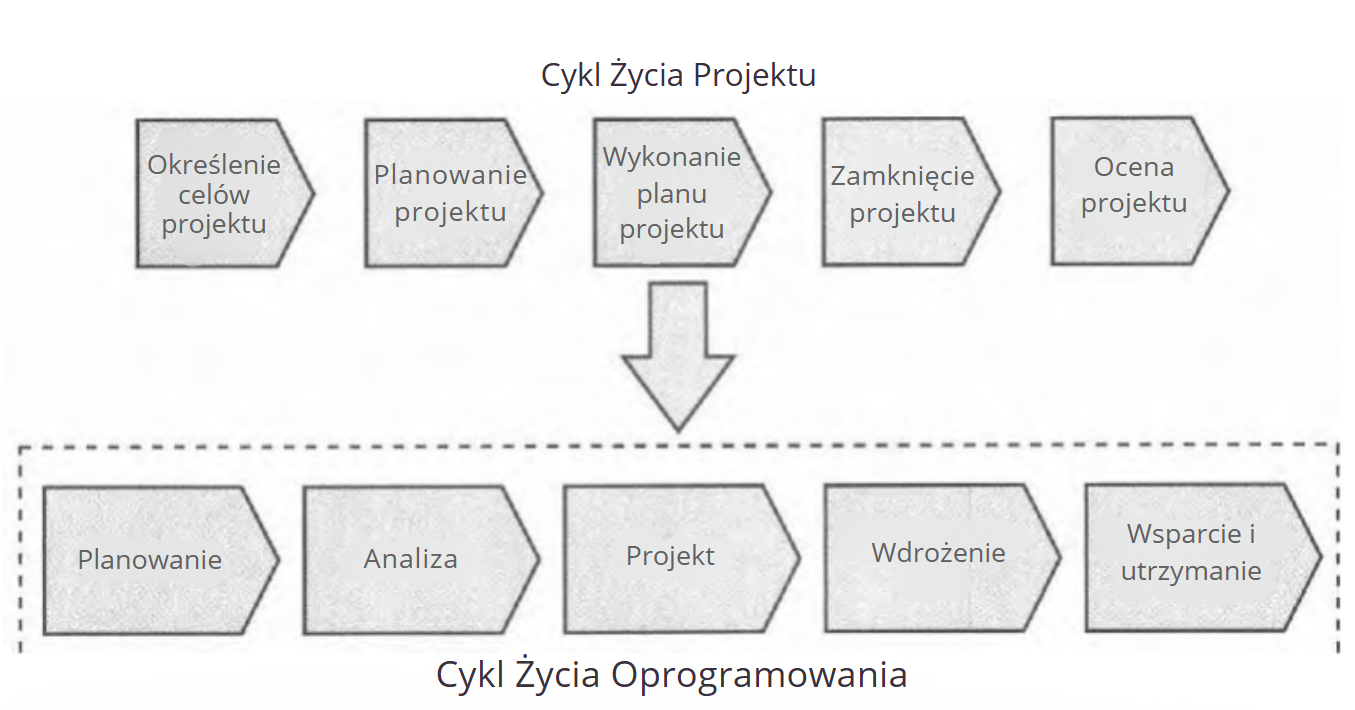
\includegraphics[width=1\linewidth]{img/plc_PL.png}
    \caption*{J. T. Marchewka. Information Technology Project management. Northern Illinois University, 2003}
\end{figure}

\subsection{Modele SDLC}
W inżynierii oprogramowania koncepcja SDLC stanowi podstawę wielu modeli cyklu życia oprogramowania. Modele te tworzą ramy planowania i kontroli procesu tworzenia systemu informatycznego. \autocite{swebok} Wszystkie sugerowane modele SDLC dzielą podstawowe cechy: składają się z sekwencji faz lub kroków, które muszą być przestrzegane i zakończone przez programistów oraz projektantów systemów, aby osiągnąć rozwinięte systemy i dostarczyć wymagane produkty. \autocite{alshamrani2015comparison} Każdy system oprogramowania posiada unikalne cechy odzwierciedlające potrzeby interesariuszy – zarówno biznesowe, jak i techniczne. Odpowiedni cykl życia powinien uwzględniać wszystkie te wymagania. \autocite{swebok} Wybór modelu SDLC powinien być dokonywany na podstawie wymagań projektu. \autocite{arora2016analysis}

PMBOK® krótko opisuje pięć cykli życia produktu lub rozwoju. Dwa czynniki są istotne przy wyborze odpowiedniego cyklu życia: stopień zmienności wymagań oraz częstotliwość dostarczania użytecznych wyników. Na przykład, dla produktu o niskim stopniu zmienności wymagań i niskiej częstotliwości dostarczania, odpowiedni będzie cykl życia predykcyjny. \autocite{pmbok6}\autocite{ITPM}

\begin{itemize}
    \item \textbf{Cykl życia predykcyjny:} Zakres, harmonogram i koszty są określane na wczesnym etapie, a zmiany w zakresie są ściśle kontrolowane. PMI określa również cykle predykcyjne jako model kaskadowy (waterfall). \autocite{pmbok}\autocite{ITPM}
    
    \item \textbf{Cykl życia iteracyjny:} Zakres jest określany na wczesnym etapie, ale szacowania czasu i kosztów są modyfikowane w miarę wzrostu wiedzy zespołu o produkcie. Iteracje służą do rozwijania produktu poprzez powtarzające się cykle, które dodają kolejne funkcjonalności. \autocite{sommerville2015software}\autocite{farley2021}\autocite{pmbok6} Długość iteracji definiuje się dla każdego projektu. \autocite{swebok} To podejście najlepiej sprawdza się w przypadku wysokiego stopnia zmienności i niskiej częstotliwości dostarczania. \autocite{ITPM}
    
    \item \textbf{Cykl życia przyrostowy:} Produkt końcowy jest dostarczany poprzez serię iteracji stopniowo dodających funkcjonalność w określonym przedziale czasowym. Produkt osiąga pełną funkcjonalność dopiero po ostatniej iteracji. \autocite{sommerville2015software}\autocite{farley2021}\autocite{pmbok6} To podejście najlepiej sprawdza się w przypadku niskiego stopnia zmienności i wysokiej częstotliwości dostarczania. \autocite{ITPM}
    
    \item \textbf{Cykl życia adaptacyjny:} Interesariusze definiują i zatwierdzają szczegółowy zakres przed rozpoczęciem iteracji, dostarczając użyteczny produkt na końcu każdej iteracji. PMI określa również cykle adaptacyjne jako zwinne (agile) lub sterowane zmianą. To podejście najlepiej sprawdza się w przypadku wysokiego stopnia zmienności i wysokiej częstotliwości dostarczania. \autocite{pmbok6}\autocite{ITPM}
    
    \item \textbf{Cykl życia hybrydowy:} Jest to kombinacja podejścia adaptacyjnego i predykcyjnego. Oznacza to, że niektóre elementy pochodzą z podejścia predykcyjnego, a inne z podejścia adaptacyjnego. Takie podejście do rozwoju jest przydatne, gdy istnieje niepewność lub ryzyko związane z wymaganiami. Hybrydowe podejście sprawdza się również, gdy dostarczane elementy mogą być modularne lub gdy różne zespoły projektowe mogą opracowywać różne części produktu. Podejście hybrydowe jest bardziej adaptacyjne niż podejście predykcyjne, ale mniej niż podejście w pełni adaptacyjne. \autocite{pmbok7}
\end{itemize}

Kilka modeli cyklu życia stało się dobrze znanych wraz z rozwojem inżynierii oprogramowania od jej początków, dwa z nich zostaną omówione w kolejnych podrozdziałach.

\subsubsection{Model kaskadowy}

Jednym z modeli, który zdobył popularność we wczesnej historii dyscypliny inżynierii oprogramowania, jest model kaskadowy. \autocite{sommerville2015software} Model kaskadowy, zaliczany do modeli predykcyjnych, zakłada określenie zakresu, harmonogramu i kosztów już na wczesnym etapie, a wszelkie zmiany są ściśle kontrolowane. Podejście to obejmuje fazy takie jak: zbieranie wymagań, projekt wstępny, projekt szczegółowy, kodowanie oraz testowanie, przy czym kolejna faza nie może się rozpocząć, dopóki poprzednia nie zostanie zakończona. \autocite{swebok} Po zakończeniu fazy nie wracamy już do niej, dlatego model ten jest zazwyczaj planowany przy użyciu wykresu Gantta. Podstawowe założenie metody kaskadowej polega na zapewnieniu stabilności wymagań. Wymagania określają potrzebne informacje, funkcje, zachowanie, wydajność oraz interfejsy. \autocite{arora2016analysis}

Postęp w modelu kaskadowym przebiega z góry na dół, przypominając wodospad. Model ten wywodzi się z przemysłu produkcyjnego oraz budownictwa, czyli silnie ustrukturyzowanych środowisk fizycznych, w których wprowadzanie zmian po fakcie jest niezwykle kosztowne, a często wręcz niemożliwe. Ponieważ w tamtym czasie nie istniały formalne metodologie tworzenia oprogramowania, ten produkcyjny model został po prostu zaadaptowany do potrzeb rozwoju oprogramowania. \autocite{SDLC}

Pierwszy formalny opis modelu kaskadowego często przypisuje się artykułowi opublikowanemu w 1970 roku przez Winstona W. Royce'a (1929–1995), \autocite{royce1970} chociaż w swoim artykule nie użył on terminu „waterfall” (kaskadowy). Royce przedstawił ten model jako przykład wadliwego, nieskutecznego podejścia. W rzeczywistości właśnie w ten sposób termin ten był najczęściej używany w literaturze dotyczącej inżynierii oprogramowania – jako sposób na krytykę powszechnie stosowanej praktyki wytwarzania oprogramowania. \autocite{SDLC}

Model kaskadowy był jednak użyteczny, gdyż wprowadził systematyzację w rozwoju systemów oprogramowania, czyli inżynierskie podejście do tworzenia produktów programistycznych. \autocite{swebok}

\textbf{Zalety podejścia kaskadowego}
\begin{itemize}
    \item Proste i łatwe w użyciu oraz zrozumieniu.
    \item Fazy nie nakładają się na siebie, co pozwala na efektywne zarządzanie projektem.
    \item Bardzo dobrze sprawdza się w małych projektach.
\end{itemize}

\textbf{Wady podejścia kaskadowego}
\begin{itemize}
    \item Nie można uzyskać akceptacji użytkownika aż do zakończenia całego procesu.
    \item Sukces projektu jest niepewny aż do jego zakończenia.
\end{itemize}

\textbf{Kiedy stosować metodę kaskadową}
\begin{itemize}
    \item Model najlepiej sprawdza się, gdy wszystkie wymagania są jasne, stałe i dobrze określone.
    \item Definicja produktu i wykorzystywana technologia są dobrze znane.
    \item Brak niejednoznacznych wymagań.
    \item Czas trwania projektu jest krótki. \autocite{arora2016analysis}
\end{itemize}

\subsubsection{Agile}

Kolejnym popularnym modelem jest agile. Jest to model iteracyjny, w którym fazy projektu przebiegają równocześnie, tj. równolegle. Wymagania mogą ewoluować na każdym etapie i w każdej fazie. \autocite{arora2016analysis}

Manifest Agile \autocite{agileManifesto} wywołał rewolucję w społeczności inżynierii oprogramowania, wprowadzając przekonanie, że proces powinien być otwarty na zmiany – wymagania mogą być modyfikowane na każdym etapie, jeśli zmienią się potrzeby użytkowników. Kluczowe stały się komunikacja i wzajemne zaufanie między zespołem a klientem. Sygnatariusze Manifestu podkreślali, że choć komunikacja (często twarzą w twarz) i interakcje z klientem są niezwykle istotne, dokumentacja (np. do definiowania wymagań) pozostaje konieczna. Postulowali także małe, przyrostowe dostawy oprogramowania, w przeciwieństwie do modelu kaskadowego, gdzie całość produktu dostarczana jest dopiero na zakończenie projektu. \autocite{swebok}

\begin{figure}
    \centering
    \caption{Wartości Agile}
    
\includegraphics[width=1\linewidth]{img/agile2.png}
    \caption*{Żródło: https://www.intellect.pl/blog/dlaczego-agile/}
\end{figure}

Agile wyraźnie rozróżnia wartości i zasady (np. ciągłe dostarczanie wartości czy zobowiązanie do doskonałości technicznej) od praktyk (takich jak programowanie w parach, planowanie sprintów czy retrospektywy). 
Mentalność Agile, oparta na zasadach takich jak otwartość na zmiany i nacisk na komunikację, różni się od podejścia predykcyjnego, które skupia się na realizacji ustalonych specyfikacji wymagań. Agile pomaga również radzić sobie ze złożonością systemów. \autocite{swebok}

Możemy postrzegać metody zwinne, takie jak Extreme Programming (XP) i Scrum, jako reakcję na modele predykcyjne, które kładą nacisk na "zracjonalizowane, inżynierskie podejście", \autocite{dyba2000} obejmujące szczegółowe planowanie, sformalizowane procesy oraz rygorystyczne wykorzystanie komponentów. \autocite{boehm2002} W przeciwieństwie do nich, metody zwinne odpowiadają na wyzwania nieprzewidywalnego świata, podkreślając wartość, jaką ludzie i ich relacje wnoszą w rozwój oprogramowania. \autocite{dyba2009we}\autocite{nerur2007}

Wokół Agile narosło wiele nieporozumień. Niektórzy myślą, że Agile stanowi kompletną metodę – jednak nie jest ona metodą samą w sobie, lecz zbiorem wartości, zasad i praktyk. Inne błędne przekonanie mówi, że Agile jest szybszy niż model kaskadowy, gdyż nie wymaga tworzenia dokumentacji. Kolejnym mitem jest pogląd, że Agile opiera się na ograniczonym zbiorze metod. 
Mimo rosnącej popularności modelu Agile, skalowanie go na duże projekty i portfele pozostaje wyzwaniem. Obecnie uważa się, że Manifest Agile przyniósł znaczące zmiany, jednak po 20 latach niektórzy autorzy sugerują konieczność aktualizacji pewnych jego zasad. \autocite{swebok}

Agile to nie tylko zbiór technik programistycznych, ale "ruch, ideologia, filozofia". Idąc jeszcze dalej, jeden z twórców Scruma stwierdza: „Agile to emocja”. \autocite{meyer2014agile} Zastosowanie praktyk Agile wykracza poza sam proces inżynierii oprogramowania – terminy takie jak „zwinność biznesowa” oraz „zwinne organizacje” stały się powszechne. Z perspektywy inżynierii oprogramowania Agile umożliwił ponowną inżynierię i lepsze dopasowanie procesów technicznych do strategicznych celów biznesowych. Wykorzystanie podejścia Agile w procesach biznesowych znajduje odzwierciedlenie między innymi w zasadach DevOps oraz w procesach oceny i doskonalenia jakościowych. \autocite{swebok}

\textbf{Zalety podejścia Agile}
\begin{itemize}
    \item Zmiany można wprowadzać bardzo łatwo.
    \item Zmiany można obsłużyć bez dużych kosztów ponownego planowania.
    \item Stałe zaangażowanie zespołu.
\end{itemize}

\textbf{Wady podejścia Agile}
\begin{itemize}
    \item Częściej pojawiają się problemy ze strukturą zespołu niż problemy z planowaniem.
    \item Niepewne terminy planowania.
\end{itemize}

\textbf{Kiedy stosować podejście Agile}
\begin{itemize}
    \item Gdy istnieje ciągła potrzeba wprowadzania zmian.
    \item Gdy zarówno programiści, jak i inni interesariusze mają swobodę sugerowania zmian. \autocite{arora2016analysis}
\end{itemize}

\begin{figure}
    \centering
    \caption{Porównanie modelu kaskadowego z Agile}
    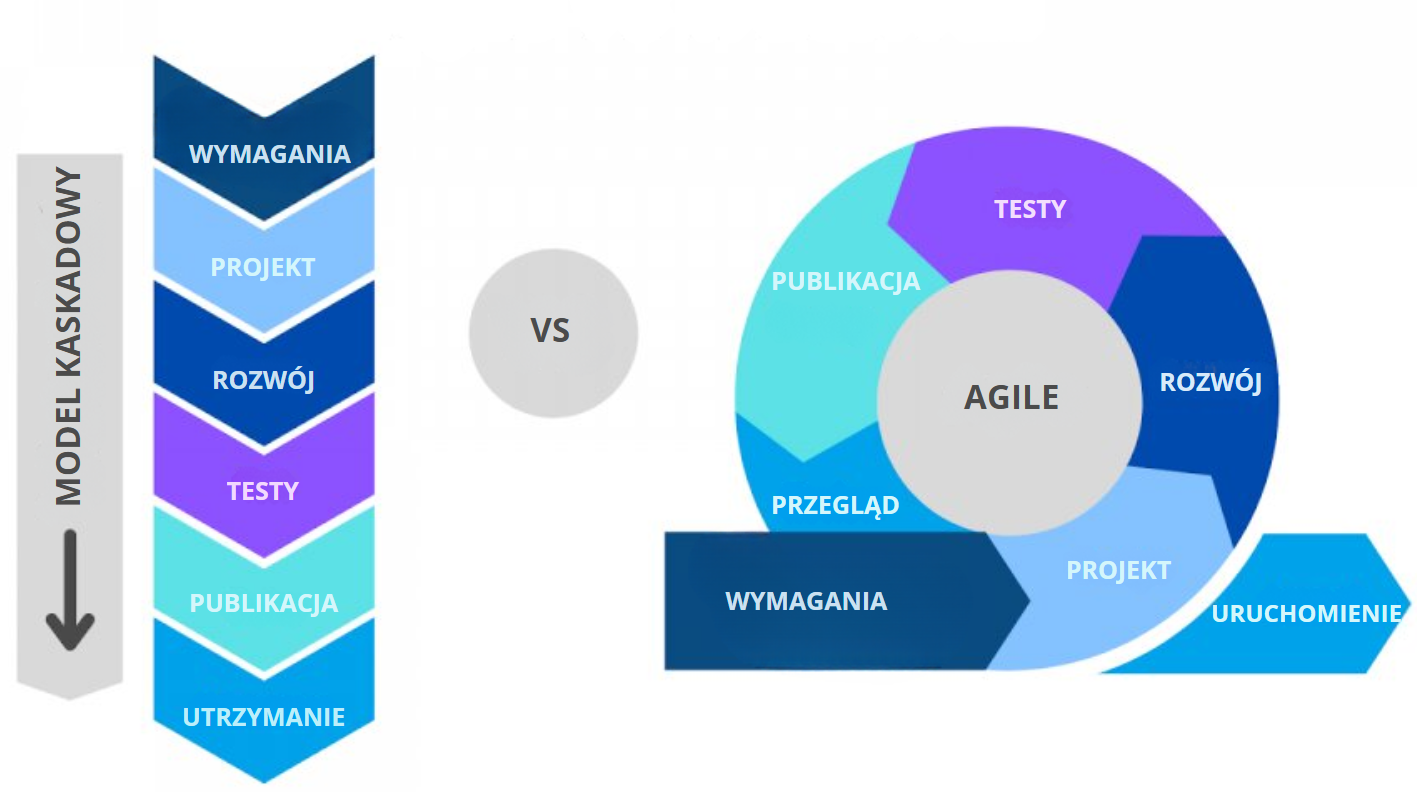
\includegraphics[width=1\linewidth]{img/waterfall_agile_PL.png}
    \caption*{Żródło: https://www.linkedin.com/pulse/waterfall-vs-agile-which-better-you-why-datacademy-cloud/}
\end{figure}

\subsection{Różnorodne technologie}
Różnorodność technologii w branży IT jest bardzo duża i kompetencje oraz wiedza specjalistów mogą się bardzo różnić pomiędzy zajmowanymi stanowiskami. 
Różnice te często znacznie utrudniają komunikację nawet wewnątrz zespołu projektowego. Na przykład:
\begin{itemize}
    \item Specjaliści od sprzętu mogą nie rozumieć języka analityków baz danych i odwrotnie.
    \item Eksperci ds. bezpieczeństwa mogą mieć trudności w dialogu z analitykami biznesowymi.
\end{itemize}

Nawet osoby pracujące w tej samej dziedzinie IT czasem się nie rozumieją, jeśli korzystają z innych technologii. Przykładowo, jeśli programista jest specjalistą w języku Java, to może mieć problem ze zrozumieniem pewnych zagadnień charakterystycznych dla języka Python, co ponownie może powodować zakłócenia w komunikacji.

Kolejnym wyzwaniem związanym z różnorodnością technologii jest ich szybka zmienność. Zespół może być bliski ukończenia projektu, gdy odkryje nowe rozwiązanie, które znacząco ulepszy produkt i lepiej zaspokoi długoterminowe potrzeby biznesowe. Nowe technologie skróciły też czas, jaki firmy mają na opracowanie, wdrożenie i dystrybucję produktów czy usług. To dynamiczne środowisko wymaga równie szybkich procesów zarządzania projektami IT. \autocite{ITPM}

\subsection{Specjaliści IT}
Inwestycje w technologie informatyczne są ściśle związane z rosnącym zapotrzebowaniem na wykwalifikowanych pracowników. Innymi słowy, jednym z głównych czynników sukcesu projektów IT są umiejętności techniczne zespołu. Według Tohidi specjaliści IT są zazwyczaj silni w dziedzinie podejmowania decyzji, jednak mają oni często duże braki komunikacyjne. Większość z nich jest introwertykami i brakuje im umiejętności, takich jak:
\begin{itemize}
    \item Umiejętności wsparcia: Przyjazne i taktowne podejście, cierpliwość, empatia wobec osób zestresowanych lub mających obawy, wysłuchiwanie skarg i problemów oraz uwzględnianie potrzeb innych.
    \item Szkolenie i doradztwo: Dostarczanie szkoleń i praktycznych porad, tworzenie kontekstu ułatwiającego rozwój umiejętności, wspieranie przedsiębiorczości i optymalizacja procesów biznesowych.
    \item Zarządzanie postawami i budowanie zespołu: Rozwiązywanie konfliktów, motywowanie do współpracy, identyfikowanie kluczowych obszarów biznesowych.
    \item Networking: Nieformalna komunikacja z osobami posiadającymi wartościowe informacje, utrzymywanie regularnych kontaktów (spotkania, rozmowy telefoniczne, korespondencja) oraz uczestnictwo w wydarzeniach społecznych.
\end{itemize}

Według badań komunikacja ma zaś bezpośrednie przełożenie na sukces projektu. \autocite{komunikacja} Nawet technicznie doskonałe inicjatywy często upadają z powodu jej braku. \autocite{Tohidi}

\subsection{Ryzyka w projektach IT}
Wszystkie projekty są ryzykowne, ponieważ stanowią unikalne przedsięwzięcia o różnym stopniu złożoności, których celem jest dostarczanie korzyści. Realizowane są one w kontekście ograniczeń i założeń, przy jednoczesnym uwzględnianiu oczekiwań interesariuszy, które mogą być sprzeczne i zmienne. Organizacje powinny podejmować ryzyko projektowe w sposób kontrolowany i świadomy, aby tworzyć wartość, równoważąc ryzyko i zysk. \autocite{pmbok6}

Niepewność to brak zrozumienia i świadomości w zakresie problemów, zdarzeń, ścieżek działania lub rozwiązań do wdrożenia. Ryzyko zaś jest aspektem niepewności. Ryzyko definiuje się jako niepewne zdarzenie lub warunek, które w przypadku wystąpienia może wywrzeć pozytywny lub negatywny wpływ na jeden lub więcej celów projektu. Ryzyka negatywne nazywane są zagrożeniami, zaś pozytywne – szansami. Wszystkie projekty obarczone są ryzykiem, ponieważ są to unikalne przedsięwzięcia charakteryzujące się różnym stopniem niepewności. \autocite{pmbok7}

Projekty informatyczne niosą za sobą pewne specyficzne dla nich aspekty ryzyka, takie jak skłonność inżynierów do dodawania niepotrzebnych funkcji (ang. feature creep) czy ryzyka związane z niematerialnym charakterem oprogramowania. Szczególną uwagę należy poświęcić ryzykom związanym z wymaganiami jakościowymi oprogramowania, takimi jak bezpieczeństwo funkcjonalne (ang. safety) czy bezpieczeństwo IT (ang. security). \autocite{program}\autocite{swebok}

Poniżej została przedstawiona przykładowa propozycja kwestionariusza ryzyk dla projektu informatycznego, ryzyka zostały podzielone na pięć kategorii: \autocite{ITPM}

\begin{itemize}
    \item Ryzyko rynkowe:
    \begin{itemize}
        \item Czy projekt IT, który ma stworzyć nowy produkt lub usługę, będzie przydatny dla organizacji lub nadający się do sprzedaży?
        \item Czy użytkownicy zaakceptują i będą korzystać z produktu/usługi?
        \item Czy konkurencja nie opracuje lepszego rozwiązania szybciej, czyniąc projekt stratą czasu i pieniędzy?
    \end{itemize} 
    \item Ryzyko finansowe:
    \begin{itemize}
        \item Czy organizacja może sobie pozwolić na realizację projektu?
        \item Jak bardzo interesariusze ufają prognozom finansowym?
        \item Czy projekt spełni szacunki dotyczące wartości bieżącej netto (NPV), zwrotu z inwestycji (ROI) i okresu zwrotu?
        \item Jeśli nie, czy organizacja będzie w stanie kontynuować projekt?
        \item Czy ten projekt to najlepsze wykorzystanie środków finansowych organizacji?
    \end{itemize} 
    \item Ryzyko technologiczne:
    \begin{itemize}
        \item Czy projekt jest wykonalny technicznie?
        \item Czy wykorzysta technologie dojrzałe, nowoczesne czy eksperymentalne?
        \item Kiedy zapadną decyzje dotyczące wyboru technologii?
        \item Czy sprzęt, oprogramowanie i sieci będą działać prawidłowo?
        \item Czy technologia będzie dostępna na czas, aby osiągnąć cele projektu?
        \item Czy technologia zdezaktualizuje się, zanim powstanie użyteczny produkt?
    \end{itemize}
    \item Ryzyko kadrowe:
    \begin{itemize}
        \item Czy organizacja ma pracowników z odpowiednimi kompetencjami, aby pomyślnie zrealizować projekt?
        \item Jeśli nie, czy można znaleźć takie osoby?
        \item Czy zespół posiada umiejętności menedżerskie i techniczne?
        \item Czy członkowie zespołu mają wystarczające doświadczenie?
        \item Czy kierownictwo wyższego szczebla wspiera projekt?
        \item Czy istnieje rzecznik projektu (ang. project champion)?
        \item Czy organizacja zna sponsora/klienta projektu?
        \item Jak dobra jest relacja ze sponsorem/klientem?
    \end{itemize}
    \item Ryzyko strukturalne/procesowe:
    \begin{itemize}
        \item Na jakim poziomie zmiany wprowadzi projekt w obszarach użytkowników i procedurach biznesowych?
        \item Ile różnych grup użytkowników musi zadowolić projekt?
        \item Z iloma innymi systemami musi współdziałać nowy projekt/system?
        \item Czy organizacja ma wypracowane procesy umożliwiające sukces projektu?
    \end{itemize}
\end{itemize}

\subsubsection{Czasowy model ryzyk}
Ciekawa interpretacja i zrozumienie ryzyk w projektach informatycznych zostało zawarte w pracy Gemino. \autocite{ryzyka} Zwraca on uwagę na czasowy charakter projektów (rozumiany jako przejście od warunków początkowych, przez przebieg projektu, aż do jego rezultatów). Dzięki czemu proponuje inną formę kategoryzacji ryzyk w projektach informatycznych, uwzględniającą różnice między ryzykami obecnymi w momencie definiowania projektu a tymi, które pojawiają się lub są ujawniane podczas jego realizacji.

\textbf{Ryzyka a priori}\\
Niektóre cechy projektu, takie jak budżet, czas trwania, złożoność techniczna, niepewność wymagań, brak doświadczenia zespołu oraz niewystarczająca wiedza sponsora projektu, mogą być oszacowane przed rozpoczęciem projektu. Są to ryzyka a priori. Można wyróżnić dwie kategorie ryzyk a priori:
\begin{itemize}
    \item Ryzyka związane z elementami strukturalnymi projektu (np. czas trwania, budżet, nakład pracy, złożoność techniczna)
    \item Ryzyka wynikające z wiedzy dostępnej dla zespołu (np. kompetencje kierownika projektu, sponsora, członków zespołu)
\end{itemize}

Elementy strukturalne, takie jak wielkość projektu i złożoność techniczna, są uznawane za istotne ryzyka. \autocite{mcfarlan}\autocite{zmud} Są one znane a przynajmniej potencjalnie możliwe do określenia na początku projektu. Zarządzanie nimi wymaga stosowania tradycyjnych ("twardych") technik zarządzania projektami, takich jak podział pracy, estymacja, harmonogramowanie oraz budżetowanie.

Brak zasobów wiedzy (np. niedoświadczony kierownik projektu lub zespół) jest również ważną kategorią ryzyk w projektach informatycznych. \autocite{mcfarlan}\autocite{barki} Ryzyka te wymagają zastosowania technik zarządzania, które często określa się mianem „umiejętności miękkich”, takich jak komunikacja, budowanie zespołu, uczenie się i koordynacja wiedzy. 

\textbf{Ryzyka wyłaniające się}\\
Zanim projekt się rozpocznie, kierownik projektu wyrabia sobie oczekiwania co do poziomu wsparcia ze strony najwyższego kierownictwa oraz użytkowników. Jednakże oczekiwany poziom wsparcia lub uczestnictwa nie wpływa bezpośrednio na wyniki projektu. To właśnie rzeczywisty poziom wsparcia, ujawniony przez zachowania najwyższego kierownictwa i użytkowników, ma najbardziej bezpośredni wpływ na efektywność. \autocite{chaos} Na przykład, choć kierownik projektu może wierzyć, że otrzyma wysoki poziom uczestnictwa użytkowników, to rzeczywisty poziom uczestnictwa ujawnia się dopiero poprzez zachowania użytkowników w trakcie realizacji projektu. Kierownik wyższego szczebla może obiecywać wysoki poziom wsparcia, ale nie dostarczyć go w praktyce. Dlatego te ryzyka można określić jako ryzyka wyłaniające się (ang. Emergent Risks).

Można wyróżnić dwie kategorie ryzyk wyłaniających się:
\begin{itemize}
    \item Ryzyka związane z niedoborami wsparcia organizacyjnego (np. brak wsparcia sponsora, klienta lub użytkownika)
    \item Ryzyka związane ze zmianami, które zachodzą (np. zmiany celów, członków zespołu oraz szerszego otoczenia)
\end{itemize} \autocite{ryzyka}

Pierwszą z tych kategorii to ryzyko wsparcia organizacyjnego. Istnieją trzy kluczowe obszary wsparcia organizacyjnego — wsparcie sponsora wykonawczego, zaangażowanie menedżera klienta oraz uczestnictwo użytkowników. Wsparcie organizacyjne jest uznawane za kluczowe dla sukcesu projektu. Gdy poziom wsparcia organizacyjnego jest niższy niż oczekiwano, określa się to jako ryzyko (np. brak wsparcia ze strony kierownictwa). Natomiast gdy wsparcie organizacyjne spełnia lub przewyższa oczekiwania, traktuje się je jako istotny zasób dla kierowników projektów. \autocite{keil}\autocite{sharma}\autocite{yetton}

Drugą kategorię ryzyk stanowią zmiany wpływające na projekty, w tym zmiany celów projektu, kluczowych osób oraz warunków zewnętrznych, z którymi projekt musi się mierzyć. Są to ryzyka zmienności projektu. \autocite{gemino} Kategoria ta jest podobna do kategorii ryzyka „środowiskowego” zidentyfikowanej przez Keil. \autocite{keil} Ta zmienność często pozostaje poza kontrolą członków zespołu projektowego, ale może mieć znaczący wpływ na wyniki projektu. \autocite{ryzyka}

Omówione kategorie ryzyk zostały przedstawione w tabelach 4.1. oraz 4.2.

\begin{table}
    \caption{Kategoryzacja ryzyk według modelu czasowego}
    \centering
    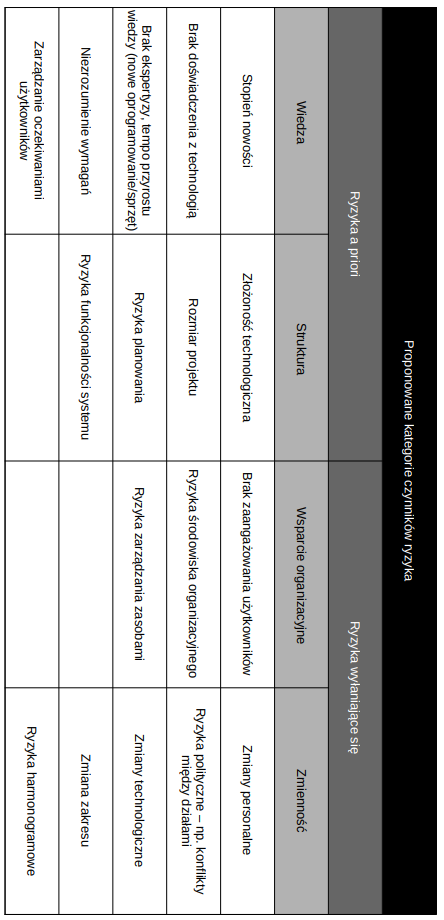
\includegraphics[width=0.5\linewidth]{img/ryzyka3.png}
    \caption*{Źródło: Gemino, Reich i Sauer, „A Temporal Model of Information Technology Project Performance” }
  \end{table}

\subsection{Ewaluacja projektów informatycznych}
Szybkie tempo zmian w technologii IT powoduje poważne trudności już na etapie rozpoczynania każdej dużej inwestycji. Każdy długoterminowy, sztywny projekt staje się niemal przestarzały, zanim w ogóle się rozpocznie, a w momencie pełnej instalacji jest już z pewnością nieaktualny. Nie oznacza to jednak, że nie należy dokonywać oceny projektów. Ocenianie lub uzasadnianie inwestycji w technologię informacyjną jest problematyczne. Inwestycje w technologię informacyjną są trudniejsze niż wiele innych decyzji inwestycyjnych, ponieważ koszty i korzyści trudno jest zidentyfikować i zmierzyć, a występujące czynniki niematerialne mogą mieć istotne znaczenie. \autocite{powell1992information}

Czasami wartość projektu informatycznego nie jest od razu znana w momencie wdrożenia systemu. Na przykład, celem projektu mającego na celu stworzenie witryny e-commerce powinno być generowanie zysków – a nie budowanie lub instalacja sprzętu, oprogramowania i stron internetowych na określonej platformie serwerowej. Technologia i jej późniejsze wdrożenie są jedynie środkiem do osiągnięcia celu. W związku z tym celem witryny e-commerce może być wygenerowanie 250 000 dolarów w ciągu sześciu miesięcy. W rezultacie ocena, czy projekt osiągnął swój cel, może nastąpić dopiero po wdrożeniu systemu. \autocite{ITPMMarchewka}

Komitety oceniające w organizacjach często stają przed wyborem, w którym konkurencyjne technologie nie dają się łatwo ze sobą porównać. Wynika to z faktu, że dwa projekty mogą zaspokajać różne, a nawet konkurencyjne wymagania. Ostateczna pozycja w rankingu technologii zależy od tego, w jakim stopniu każda z nich odpowiada na poszczególne wymagania. Jednak poza przypadkami, w których jedna technologia wyraźnie dominuje pozostałe, pojawia się problem, gdy dwie alternatywy zaspokajają odmienne i konkurencyjne potrzeby. Rozwiązanie takich konfliktów jest praktycznie niemożliwe bez udziału wiedzy eksperckiej w procesie podejmowania decyzji. \autocite{thomaidis2006evaluation}

Currie określa jednak uzasadnianie inwestycji w IT jako „rytuał legitymizacji”, a nie proces rzeczywistej oceny korzyści. \autocite{Currie1989} Jak zauważył Williams już pół wieku temu: „W biznesie nie chodzi o to, by tworzyć dobre prognozy, lecz by sprawiać, aby się one spełniały”. \autocite{williams1967technology}

\subsection{Ostatnie trendy w projektach informatycznych}
Ostatnie trendy, takie jak rosnąca globalizacja, outsourcing oraz zespoły wirtualne, stwarzają nowe wyzwania i możliwości dla kierowników projektów informatycznych oraz ich zespołów. \autocite{ITPM}

\subsubsection{Globalizacja}
Globalizacja to termin powszechnie używany, lecz o niejasnym znaczeniu, nawet wśród tych, którzy się nim posługują. \autocite{robertson2007globalization} Anthony McGrew twierdzi, że globalizacja stanowi sieć powiązań i połączeń wykraczających poza państwa narodowe (a tym samym społeczeństwa), które tworzą współczesny system światowy. To proces, w ramach którego wydarzenia, decyzje i działania w jednej części świata mogą mieć znaczące konsekwencje dla jednostek i społeczności w odległych regionach globu. \autocite{McGrew1990}

Globalizacja znacząco wpłynęła na sektor IT. Mimo że główne firmy technologiczne, takie jak Microsoft czy IBM, powstały w Stanach Zjednoczonych, większość ich działalności ma charakter globalny – przedsiębiorstwa i osoby z całego świata przyczyniają się do rozwoju technologii informacyjnych oraz współpracują przy różnych projektach IT. \autocite{ITPM}

Ma to również znaczący wpływ na pracę kierowników projektów, gdyż muszą oni uwzględnić następujące zagadnienia:

\begin{itemize}
  \item \textbf{Komunikacja}:  
  Praca w różnych strefach czasowych, różne języki, pochodzenie kulturowe i święta wymagają efektywnego planowania komunikacji.
  \item \textbf{Zaufanie}:  
  Zaufanie jest kluczowe dla wszystkich zespołów, zwłaszcza globalnych. Należy je budować od początku, szanując różnice i doceniając wartości, jakie członkowie wnoszą do projektu.
  \item \textbf{Wspólne praktyki pracy}:  
  Należy ujednolicić procesy pracy i wypracować praktyki akceptowane przez wszystkich. \autocite{ITPM}
\end{itemize}

\subsubsection{Outsourcing}
Outsourcing oznacza pozyskiwanie dóbr i usług przez organizację z zewnętrznych źródeł. Termin offshoring odnosi się do outsourcingu realizowanego w innym kraju. Offshoring jest naturalną konsekwencją globalizacji. Projekty IT coraz częściej opierają się na outsourcingu, zarówno w granicach kraju, jak i poza nimi. Niektóre organizacje utrzymują konkurencyjność, strategicznie wykorzystując outsourcing. Wielu firmom udało się obniżyć koszty dzięki tej praktyce, mimo że bywa ona niepopularna w ich krajach macierzystych. \autocite{ITPM} Słynnym przykładem outsourcingu jest decyzja Eastmana Kodaka o przekazaniu całego centrum danych firmie IBM, operacji mikrokomputerowych Businessland oraz sieci telekomunikacyjnych i danych Digital Equipment Corporation oraz IBM.

Outsourcing IT zależy od wielu czynników na różnych poziomach. Na poziomie gospodarczym trendy i cykle ekonomiczne mogą motywować firmy do racjonalizacji zarządzania infrastrukturą IT poprzez outsourcing. Na poziomie branżowym presja konkurencyjna skłania firmy do budowania „partnerskich relacji” z kluczowymi dostawcami IT. Na poziomie firmy poszukiwanie przewagi konkurencyjnej jest kluczowym impulsem do decyzji o outsourcingu. Wewnątrz firmy decyzja o outsourcingu może zależeć od czynników menedżerskich, takich jak dążenie do kontroli zasobów lub postrzeganie informacji jako źródła władzy. \autocite{loh1992determinants}\autocite{Kanter1979}\autocite{Mintzberg1983}

W związku z rosnącym wykorzystaniem outsourcingu w projektach IT, kierownicy projektów muszą lepiej zrozumieć globalne i zamówieniowe aspekty, w tym pracę z zespołami zdalnymi. \autocite{ITPM}  

\subsubsection{Zespoły zdalne}
Globalizacja projektów zwiększyła zapotrzebowanie na zespoły zdalne, \autocite{pmbok6} czyli grupy osób współpracujących pomimo granic czasowych i przestrzennych, wykorzystujące technologie komunikacyjne. Członkowie zespołu mogą pracować dla tej samej firmy w jednym kraju lub obejmować pracowników, niezależnych konsultantów, dostawców, a nawet wolontariuszy z całego świata. \autocite{ITPM}

W konkurencyjnym rynku zespoły zdalne stanowią coraz częstsze rozwiązanie odpowiadające na potrzebę skrócenia czasu wprowadzenia produktu na rynek, obniżenia kosztów oraz szybkiego rozwiązywania złożonych problemów organizacyjnych. Zespoły wirtualne umożliwiają organizacjom łączenie talentów i ekspertyzy pracowników oraz osób z zewnątrz poprzez eliminację barier czasowych i przestrzennych. Obecnie firmy intensywnie inwestują w zespoły zdalne, aby podnieść swoją wydajność i konkurencyjność. \autocite{ebrahim2009virtual}

\textbf{Zalety zespołów wirtualnych}  
\begin{itemize}
  \item \textbf{Obniżenie kosztów} – wielu pracowników zdalnych nie wymaga biur ani dodatkowego wsparcia.
  \item \textbf{Dostęp do ekspertyzy i elastyczność} – globalny zasięg umożliwia pracę przez całą dobę, zwiększając konkurencyjność.
  \item \textbf{Lepsza równowaga praca–życie} – brak sztywnych godzin pracy i dojazdów.
\end{itemize}

\textbf{Wady zespołów wirtualnych}  
\begin{itemize}
  \item \textbf{Izolacja członków} – trudności w adaptacji do środowiska zdalnego.
  \item \textbf{Problemy komunikacyjne} – brak języka ciała i komunikacji niewerbalnej utrudnia budowanie relacji.
  \item \textbf{Ograniczenie nieformalnej wymiany informacji} – trudności w nawiązywaniu kontaktów.
  \item \textbf{Zależność od technologii} – awarie mogą sparaliżować pracę.
\end{itemize}


                            % na nowe wersje, a cały tekst pracy pozostaje nienaruszony.
\newpage
\section{Kierownik projektu}
Jako rozwinięcie części teoretycznej zarządzania projektami kluczowym jest zrozumienie roli oraz zadań kierownika projektu. Dodatkowo w literaturze przedmiotu jest dostępnych wiele badań oraz prac omawiających cechy oraz kompetencje kierownika projektu. Warto przytoczyć te teksty w celu udzielenia trafniejszej odpowiedzi na postawione w pracy pytanie.
%Kolejnym zagadnieniem, które zostanie poruszone w tym rozdziale, jest również to jak dokonywany jest wybór osoby na stanowisko kierownika projektu w organizacjach.
\\
\subsection{Kierownik projektu}
Najprostsza definicja za pomocą, której można wyjaśnić kim jest kierownik projektu to: osoba, która wyznacza proces dostarczenia zmiany i jest odpowiedzialna za zarządzanie tym procesem \autocite{Turner2016}.
Bardziej powszechne wydaje się jednak rozumienie kierownika jako podmiotu odpowiedzialnego za realizację projektu w sposób bezpieczny, zgodny z harmonogramem i budżetem oraz osiągający wymagane standardy wydajności lub jakości określone przez klienta \autocite{Sommerville}.
Nicholas i Steyn podają w swojej książce jednak bardziej metaforyczne rozumienie kierownika projektu jako swoistego spoiwa scalającego wszystkie elementy projektu oraz napędzającego jego rozwój. W ramach tej funkcji pełnione są liczne zadania, między innymi integracja, komunikacja, podejmowanie decyzji, motywowanie, propagowanie idei, działalność przedsiębiorcza oraz inicjowanie zmian. \autocite{NicholasSteyn}
Z taką definicją kierownika projektu zgadza się również Blackburn i Sarah. W swoim artykule określili kierownika projektu jako byt łączący sieć aktorów w celu realizacji wspólnego celu \autocite{BlackburnSarah}

\subsection{Role i zadania kierownika projektu}
Zgodnie z przytoczonymi definicjami kierownika projektu, jego głównym zadaniem jest zapewnienie dostarczenia końcowego produktu w ramach przyjętego budżetu i ustalonych terminów, zgodnie z określonymi wymaganiami technicznymi. Pozostałe obowiązki ulegają modyfikacji w zależności od umiejętności kierownika, etapu realizacji przedsięwzięcia, rozmiaru i charakteru projektu oraz zakresu odpowiedzialności przekazanej przez wyższe kierownictwo.
Mimo zróżnicowania kompetencji, zakres obowiązków zazwyczaj obejmuje:
\begin{itemize}
    \item Opracowanie planu działań projektowych, zadań oraz końcowych rezultatów, co obejmuje sporządzenie struktury podziału pracy, ustalenie harmonogramu i budżetu, a także koordynację zadań oraz dystrybucję zasobów. Polega to na łączeniu różnorodnych działań i rozproszonych elementów w sposób umożliwiający osiągnięcie wyznaczonych celów czasowych, budżetowych i jakościowych. Centralną funkcją kierownika projektu jest zapewnienie spójności wszystkich składników przedsięwzięcia, co umożliwia ich harmonijną współpracę zgodnie z ustalonym planem.
    \item Dobór oraz organizacja zespołu odpowiedzialnego za realizację przedsięwzięcia. Nawet przy ograniczonych formalnych uprawnieniach do podejmowania decyzji kadrowych, rola ta umożliwia wywieranie znaczącego wpływu na dokonywane wybory osób dysponujących odpowiednimi kompetencjami.
    \item Nawiązywanie kontaktów z interesariuszami oraz oddziaływanie na ich postawy. Na styku licznych kanałów informacyjnych znajduje się rola kierownika, odpowiedzialnego za zbieranie oraz dystrybucję danych – obejmujących raporty, zgłoszenia, notatki służbowe czy skargi. Przekazywane informacje są starannie opracowywane i poddawane analizie, aby wszyscy interesariusze byli rzetelnie poinformowani o założeniach dotyczących polityki, celów, budżetów, harmonogramów, wymagań, postępów prac oraz zmian w projekcie.
    \item Prowadzenie negocjacji oraz scalanie działań kierowników działów, wykonawców, użytkowników i kadry zarządzającej. Istotnym aspektem działalności kierownika jest również propagowanie idei projektu, co wiąże się z kreowaniem przekonania o jego wartości i wykonalności. W początkowej fazie koncepcyjnej to właśnie kierownik często dysponuje pełnym obrazem przedsięwzięcia, a jego zdolność do zdobycia poparcia kluczowych interesariuszy może przesądzić o uzyskaniu niezbędnego finansowania
    \item Zapewnienie kanału komunikacji z klientem. Znaczenie tej komunikacji podkreślają w swojej pracy Turner i MUller \autocite{turnermuller}. Przypominają oni, że kierownik projektu działa tak naprawdę w imieniu i na rzecz klienta, a więc projekt powinien być zgodny z jego potrzebami.
    \item Nadzór nad postępem realizacji projektu. Ocena rzeczywistych osiągnięć technicznych w porównaniu z planowanymi, przegląd i weryfikacja zasadności celów technicznych, potwierdzenie ciągłej potrzeby realizacji projektu, nadzorowanie wydatków na zasoby oraz porównanie przewidywanej wartości z poniesionymi kosztami. \autocite{Roman}\autocite{vaupel}
    \item Identyfikacja problemów o podłożu technicznym i funkcjonalnym a następnie bezpośrednie ich rozwiązywanie lub poszukiwanie adekwatnego wsparcia. Zarządzanie ryzykiem jest integralną częścią zarządzania projektem, obejmującą identyfikację, ocenę i planowanie reakcji na ryzyka w celu minimalizacji ich wpływu. W większych projektach, gdzie ryzyko i konsekwencje są znaczące, skuteczne zarządzanie ryzykiem może decydować o sukcesie lub porażce przedsięwzięcia.
    \item Radzenie sobie z sytuacjami kryzysowymi oraz rozwiązywanie pojawiających się konfliktów. Determinacja i skupienie zespołu na wspólnym celu stanowią jeden z kluczowych czynników mobilizujących do działania. W strukturze organizacyjnej projektu to właśnie kierownik odpowiada za kreowanie poczucia wspólnego kierunku i zaangażowania. Pomimo występowania licznych czynników sprzyjających motywacji, takich jak spontaniczność, osiągnięcia czy entuzjazm, utrzymanie wysokiego poziomu zaangażowania bywa trudne w długotrwałych i wymagających przedsięwzięciach. Czynniki takie jak brak wcześniejszych wzorców, praca na niepełny etat, różnorodność specjalizacji, sporadyczność kontaktów oraz dystans przestrzenny mogą znacząco wpływać na spadek motywacji. Skuteczne zarządzanie projektem wymaga jednak zdolności do budowania entuzjazmu, ducha zespołu, pewności siebie oraz dążenia do doskonałości.
    \item Sugerowanie zakończenia projektu lub zmiany kierunku działań, gdy założone cele okazują się nieosiągalne. Centralne położenie kierownika umożliwia podejmowanie decyzji związanych z alokacją zasobów, definiowaniem zakresu działań oraz równoważeniem kryteriów harmonogramu, kosztów i jakości. \autocite{NicholasSteyn}
\end{itemize}

Ciekawa interpretacja roli oraz zadań kierownika projektu została również przedstawiona na rysunku 3.1. Autorzy zwracają większą uwagę na rolę interpersonalną kierownika projektu i określają go w tym kontekście jako mentora, mediatora, psychologa i lidera.
\begin{figure}
\centering
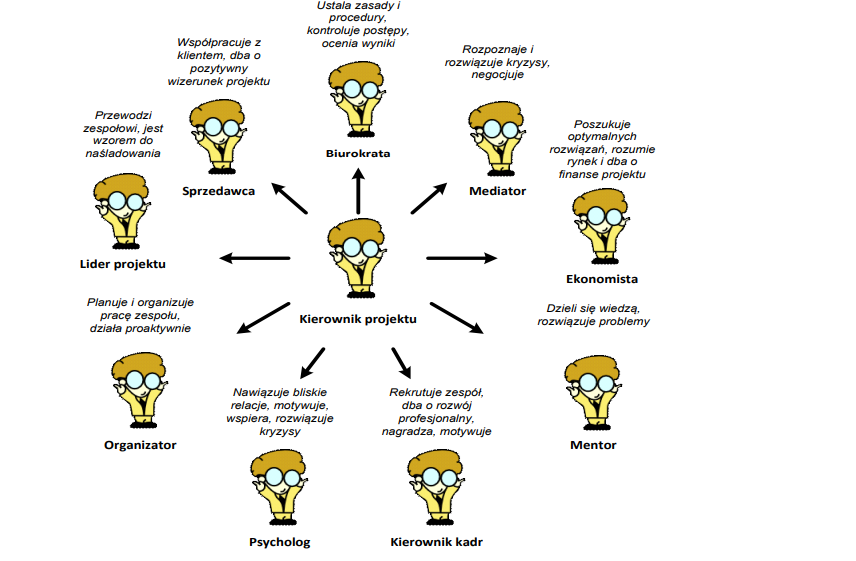
\includegraphics[width=14cm]{img/rola.png}
\caption{Źródło: R. Vaupel, G. Schmolke, A. Kruger, Customer-focused management by projects, MacMillan Publishers 2000, s.262}
\end{figure}

\subsection{Kompetencje kierownika projektu}
Dywagacje na temat kompetencji, jakie powinien posiadać kierownik projektu, stały się zagadnieniem często poruszanym w literaturze przedmiotu. Jednak nie tylko wiedza i umiejętności techniczne mają znaczenie. Menedżerowie są bardziej skłonni do osiągania lepszych wyników lub pozostawania dłużej na swoim stanowisku, jeśli ich cechy osobiste odpowiadają wymaganiom stanowiska.\autocite{MUMFORD200011}
Na rysunkach 3.2. oraz 3.3. zostały przedstawione wyniki dostępnych badań.
Na podstawie analizy dostępnej literatury i badań w dalszych sekcjach według ważności zostały wymienione kluczowe kompetencje: \autocite{analizaMulti} \autocite{Alvarenga} \autocite{arras2010} \autocite{ziek} \autocite{brill} \autocite{arras2015}

\begin{figure}
\centering
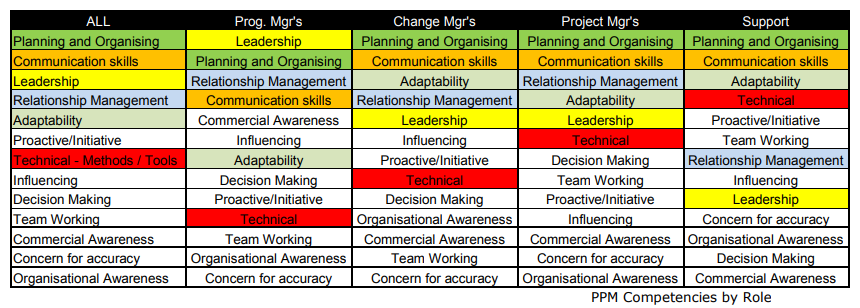
\includegraphics[width=14cm]{img/kompetencje.png}
\caption{Źródło: Arras People Project Management Benchmark Report 2010 }
\end{figure}

\begin{figure}
\centering
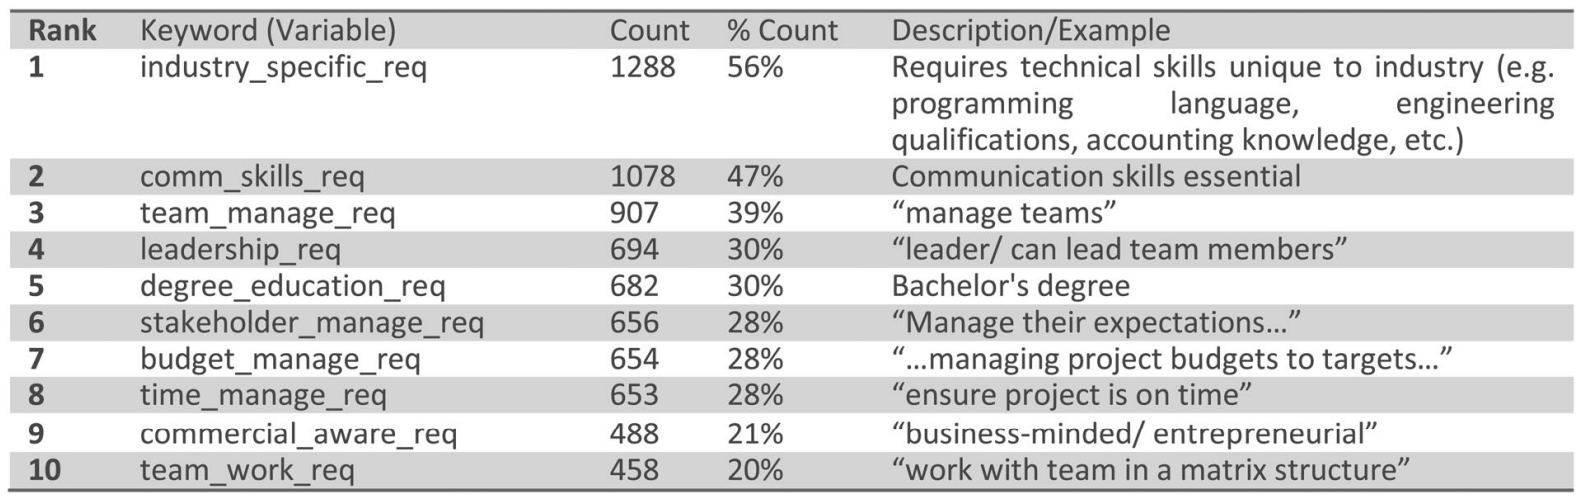
\includegraphics[width=14cm]{img/kompetencje2.png}
\caption{Źródło: A Multidimensional Analysis of ProjectManager Competences Maxwell Chipulu, Jun Guan Neoh, Udechukwu (Udi) Ojiako, and Terry Williams 2013}
\end{figure}

\subsubsection{Komunikacja}
W najnowszych badaniach oraz pracach kluczowe okazują się umiejętności interpersonalne.\autocite{brill}. Umiejętności komunikacyjne są kluczowe w różnych kontekstach: negocjacje, komunikacja, relacje z klientami i zarządzanie konfliktem. Literatura opisuje komunikację jako podstawowe narzędzie dla kierownika projektu w jego kluczowej funkcji łączenia i pośredniczenia między wieloma podmiotami zaangażowanymi w projekt: zespołem, sponsorami, sprzedawcami, kierownikami funkcjonalnymi, użytkownikami i klientami oraz innymi interesariuszami. Wyraźnie wynika z tego, że to właśnie kompetencje komunikacyjne pozwalają kierownikom projektów być skutecznymi i mieć wpływ na sukces projektu. \autocite{Alvarenga}

Ziek oraz Anderson w swojej pracy podkreślają, że rola komunikacji w projekcie to nie jest jedynie czynnik wpływający na sukces bądź porażkę projektu. Uważają oni, że jest to fundament zarządzania projektami. Zrozumienie roli komunikacji zapewnia kierownikom projektów dodatkowe środki kontroli nad projektem, wykraczające poza budżety i harmonogramy.\autocite{ziek}

\subsubsection{Przywództwo}
Podążając za Burnsem, przywództwo jest „jednym z najczęściej obserwowanych i najmniej rozumianych zjawisk na ziemi”\autocite{burns}. W związku ze skomplikowaną naturą tej cechy nie jest ona łatwa w wyjaśnieniu. Tabassi i Bakar zidentyfikowali kluczowe komponenty związane ze zjawiskiem przywództwa i zdefiniowali je jako proces, w którym lider ze swoją inteligencją i siłą woli ma wpływ na grupę podwładnych, aby móc rozwijać ich potencjały w celu osiągnięcia celów organizacyjnych w wyznaczonym czasie, finansowaniu i jakości.\autocite{Tabassi} 

Kierownik projektu nie może ograniczać się jedynie do zarządzania harmonogramem i zadaniami – kluczowe stają się rozwinięte kompetencje przywódcze, które są fundamentem sukcesu całego przedsięwzięcia. W projektach, w których nieuniknione są kryzysy i konflikty, zdolność szybkiego podejmowania decyzji oraz umiejętność skutecznego komunikowania się z zespołem nabierają szczególnego znaczenia. Nicholas podkreśla, że to właśnie przywództwo jest jedną z czterech funkcji kierownika, który ukierunkowuje pracę swoich pracowników oraz motywuje ich do realizacji wspólnego celu. \autocite{NicholasSteyn} 
W badaniu Alvarenga cechy przywódcze zostały uznane za najważniejszą kompetencję u kierownika projektu.\autocite{Alvarenga}

\subsubsection{Zarządzanie sobą (ang. Self-management)}
Kompetencje zarządzania sobą obejmują wizję, poznanie, odporność emocjonalną, samoświadomość. Odzwierciedlają one potrzebę kierowników projektów, którzy są oddani samorozwojowi i ciągłemu uczeniu się. Odporność emocjonalna jest również bardzo istotna dla kierowników projektów: ciągła presja, niepewność, ryzyko, konflikty zespołowe i inne codzienne wyzwania mogą prowadzić do stresu, a w skrajnych sytuacjach do wypalenia zawodowego.\autocite{Alvarenga} Samoświadomość oraz odporność emocjonalna są również podkreślane jako kluczowe cechy kierownika projektu w pracy Turnera i Mullera. Według ich badań samoświadomość jest zwłaszcza szczególnie ważna w projektach o średniej złożoności.\autocite{turnermuller2010}

\subsubsection{Umiejętności zarządcze}
Kierownik projektu musi zdecydować, jak przydzielić zasoby ludzkie, finansowe i informacyjne do różnych zadań projektu. Kompetencja ta opiera się na planowaniu, organizowaniu, koordynowaniu i kontrolowaniu zadań.\autocite{Gottschalk} Znaczenie tych umiejętności podkreślają również w swojej pracy Udo i Koppensteiner. Według nich kierownik projektu musi znać podstawy procesów zarządzania projektami, metodologie, narzędzia i techniki oraz potrafić dostosować je do organizacji.
Jednym ze sposobów na sprawdzenie tych kompetencji jest certyfikacja bądź odpowiednie studia.\autocite{Koppensteiner} Odpowiednie wykształcenie pojawiło się również w wynikach badań IEEE, aż 30\% respondentów uznało stopień naukowy z dziedziny zarządzania za istotną cechę kierownika projektu.\autocite{analizaMulti}

\subsubsection{Umiejętności techniczne}
Kolejną kompetencją kierownika projektu, która często pojawia się w literaturze, są umiejętności techniczne rozumiane jako wiedza domenowa oraz znajomość narzędzi potrzebnych w zarządzaniu projektami. \autocite{arras2010} \autocite{brill}
Znajomość domeny i wiedzy specyficznej dla branży jest cenna, gdyż to kierownik projektu identyfikuje potrzeby użytkowników i opracowuje rozwiązania, które zmieniają sytuacje biznesowe. Główną odpowiedzialnością kierownika projektu jest zapewnienie, że szybko planowane zmiany są zrozumiane, zaplanowane, wdrożone i strategicznie wykorzystane w organizacji.\autocite{Gottschalk} Nie byłby on w stanie tego osiągnąć bez dobrego zrozumienia projektu oraz działań wykonywanych w ramach projektu.
Ciekawym opisem poziomu kompetencji technicznych kierownika projektu jest podejście zaproponowane przez Nicholasa. Tłumaczy on, że kompetencje kierownika powinny pokrywać cały zakres projektu, ale ograniczając go jedynie do pierwszego poziomu struktury podziału pracy (ang. Work breakdown structure, WBS).\autocite{NicholasSteyn}

\subsection{Znaczenie wiedzy z zakresu inżynierii oprogramowania dla kierownika projektu}
Aby podejmować świadome decyzje, kierownicy projektów muszą rozumieć aspekty techniczne projektu. Ich kompetencje powinny obejmować pełny zakres projektu. W środowiskach nisko- lub nietechnologicznych tę znajomość można rozwijać poprzez doświadczenie i szkolenia nieformalne. W projektach o wysokim zaawansowaniu technologicznym wymagania są surowsze i zwykle obejmują karierę ukształtowaną w środowisku technologicznym oraz wiedzę z zakresu nauki lub inżynierii.

Choć kierownicy projektów rzadko przeprowadzają analizy techniczne, muszą być wykwalifikowani do podejmowania ocen technicznych oraz zdolni do analizy i integracji pracy oraz wiedzy. Wielu specjalistów technicznych nie radzi sobie dobrze ze współpracą z innymi, ponieważ większość kształcenia w dziedzinie inżynierii i technologii kładzie nacisk na analizę, pomijając umiejętności pracy zespołowej. Aby skutecznie komunikować się ze wszystkimi uczestnikami projektu i integrować ich pracę, kierownik projektu musi rozumieć i posługiwać się językiem specjalistów technicznych.\autocite{NicholasSteyn}

Z takim postrzeganiem polemizuje jednak badanie przeprowadzone wśród brazylijskich kierowników projektów informatycznych.\autocite{silva2015project} Było to jakościowe badanie eksploracyjne z udziałem 16 brazylijskich profesjonalistów IT z różnych sektorów.
Wbrew tradycyjnemu postrzeganiu w środowisku projektów informatycznych, umiejętności z zakresu inżynierii oprogramowania uznano za mniej istotne niż kompetencje behawioralne, biznesowe i menedżerskie. Analiza wykazała, że najważniejsze kompetencje to:
\begin{itemize}
    \item zarządzanie zespołem,
    \item wiedza domenowa,
    \item komunikacja,
    \item zarządzanie projektami,
    \item umiejętności interpersonalne.
\end{itemize}
\autocite{silva2015project}

Kategorie takie jak zarządzanie zespołem, wiedza domenowa, umiejętności interpersonalne i komunikacja zebrały łącznie 349 wzmianek, podczas gdy umiejętności z zakresu inżynierii oprogramowania – jedynie 5. Dla respondentów kompetencje związane z relacjami i biznesem są więc kluczowe dla sukcesu projektu informatycznego. Niektórzy zauważyli nawet, że kierownicy z silnym profilem technicznym mogą bagatelizować inne aspekty zarządzania, takie jak strategia organizacyjna, umiejętności polityczne czy zarządzanie ludźmi. W badaniu została przytoczona w tym kontekście wypowiedź respondentów:
\begin{itemize}
    \item"Był bardziej techniczny, brakowało mu wiedzy politycznej. Brakowało mu politycznej siły, by projekt działał."
    \item"Czasami kierownik z dobrymi umiejętnościami technicznymi nie skupia się na ludziach." 
\end{itemize}

Badanie jednak nie bagatelizuje całkowicie roli umiejętności z zakresu inżynierii oprogramowania, uznaje je za "niezbędne, ale niewystarczające". Niektórzy z respondentów badania podkreślali, że wiedza techniczna ułatwia komunikację z programistami oraz usprawnia zarządzanie projektem. Przytoczono w tym kontekście następujące wypowiedzi.
\begin{itemize}
    \item"Gdy masz umiejętności techniczne, możesz porozumieć się z osobą rozwijającą system i przekazać programiście oczekiwania klienta."
    \item"Jeśli kierownik nie ma wiedzy technicznej, musi stale polegać na kimś, kto ją posiada."    
\end{itemize}

Zgromadzone dane wskazują, że umiejętności z zakresu inżynierii oprogramowania nie wystarczą, aby zapewnić pozytywne rezultaty w zarządzaniu projektami. Nie oznacza to, że kierownicy projektów IT powinni porzucić kompetencje techniczne wypracowane w trakcie kariery. Sugeruje to jednak, że powinni łączyć umiejętności techniczne z kompetencjami interpersonalnymi i menedżerskimi, aby skuteczniej osiągać sukces projektu.\autocite{silva2015project}


Podobne badania przeprowadził Stevenson wśród osób odpowiedzialnych za rekrutację kierowników projektów informatycznych.\autocite{stevenson2010pm} Badanie to wykazało niską ocenę ekspertyzy technicznej jako kompetencji kierowników projektów. Biorąc pod uwagę zmiany i konsolidację ról w zespołach projektowych oraz trend wzrostowy zatrudniania kierowników o profilu technicznym w ciągu ostatniej dekady, oczekiwano, że umiejętności techniczne zostaną uznane za istotne kryterium. Jedną z interpretacji tych wyników jest to, że firmy mniej cenią kompetencje techniczne kierowników projektów zdobyte w innych firmach, a bardziej skupiają się na szkoleniu swoich pracowników wewnętrznie, w oparciu o własną technologię. Inna interpretacja zakłada, że respondenci uważali, iż podstawowy poziom wiedzy technicznej jest inherentny u wszystkich kandydatów, więc nie traktowali go jako kryterium różnicującego talenty.

Wyniki badania jednoznacznie wskazują, że kompetencje „miękkie” takie jak przywództwo, umiejętność komunikacji na wielu poziomach, zdolności werbalne i pisemne, postawa oraz zdolność radzenia sobie z niejednoznacznością i zmianami – są kluczowymi cechami, które są poszukiwane wśród kierowników projektów informatycznych i które decydują o skutecznym zarządzaniu projektami.\autocite{stevenson2010pm}

Ważność umiejętności technicznych a menedżerskich zależy od typu projektu. W projektach innowacyjnych kierownik musi mieć wyższe kompetencje techniczne ze względu na złożoność problemów i techniczne nastawienie zespołu. W projektach rozwojowych lub nietechnicznych kluczowe są zdolności menedżerskie ze względu na współpracę z wieloma obszarami funkcjonalnymi. Ogólnie rzecz biorąc, kierownicy muszą mieć wystarczające umiejętności techniczne, by rozumieć problem, choć nadmierne skupienie na umiejętnościach technicznych może prowadzić do zaniedbywania roli menedżerskiej. Nie ma jednak substytutu dla silnych kompetencji zarządczych w tej roli.

Aby sprostać wymaganiom zarówno technicznym, jak i administracyjnym, w projektach czasem zatrudnia się dwóch menedżerów: technicznego i administracyjnego. Często występuje to w projektach budowlanych, gdzie architekt odpowiada za kwestie techniczne, a tzw. kierownik projektu zajmuje się „dokumentacją administracyjną”. Obecność dwóch menedżerów komplikuje koordynację, komunikację i kwestie władzy, ponieważ obaj dzielą odpowiedzialność. Co więcej, gdy kierownik projektu jest podporządkowany architektowi, jego zdolność do zarządzania projektem jest ograniczona. Podobny podział występuje w branży filmowej: producent zarządza zasobami, harmonogramami i budżetami (pełniąc rolę kierownika projektu), podczas gdy reżyser nadzoruje kwestie techniczno-artystyczne. Ponieważ tworzenie filmu to przedsięwzięcie artystyczne, reżyserzy potrzebują elastyczności w budżetach i harmonogramach zdjęć, ale koszty również mają znaczenie – producent staje przed dylematem: „jaką cenę zapłacić za kreatywność?”.

Idealnie, projekt powinien mieć jednego kierownika, a wszyscy inni pełniący role menedżerskie lub administracyjne podlegają jemu.\autocite{NicholasSteyn} % wystarczy podmienić swoje pliki main.tex i eiti-thesis.cls
\newpage

\section*{Rozdział X: Analiza badania dotyczącego kompetencji kierownika projektu informatycznego}

\subsection*{1. Cel badania}

Celem przeprowadzonego badania było zidentyfikowanie kluczowych kompetencji, które według specjalistów z branży IT powinien posiadać skuteczny kierownik projektu informatycznego. Inspirację do konstrukcji narzędzia badawczego stanowiła klasyfikacja kompetencji zaproponowana w pracy \textcite{araujo2020it}, gdzie autorki wyróżniły pięć głównych obszarów: interpersonalne, przywódcze, strategiczne, organizacyjne oraz techniczne.

\subsection*{2. Metodologia}

Badanie zostało zrealizowane w formie anonimowej ankiety internetowej. Wzięło w nim udział 30 respondentów reprezentujących różne stanowiska w sektorze IT. Kwestionariusz zawierał pytania zamknięte z oceną w skali Likerta (1–5), a także pytania otwarte, umożliwiające rozszerzenie odpowiedzi o opinie jakościowe.

\subsection*{3. Charakterystyka próby}

Wśród respondentów dominowali programiści (20 osób), następnie kierownicy projektów (5 osób) oraz inne role (5 osób). Największa część respondentów miała od 2 do 10 lat doświadczenia zawodowego. Większość uczestników brała udział w projektach rozwojowych (25 osób) oraz utrzymaniowych (24 osoby), a 15 wskazało na doświadczenie we wdrożeniach.

\subsection*{4. Wyniki ilościowe}

\subsubsection*{4.1 Porównanie średnich ocen kompetencji}

\begin{table}[H]
\centering
\caption{Średnie oceny ważności kategorii kompetencji}
\begin{tabular}{ll}
\toprule
\textbf{Kategoria kompetencji} & \textbf{Średnia ocena (1–5)} \\
\midrule
Interpersonalne i komunikacyjne          & \textbf{4{,}71} \\
Przywódcze i zarządcze                   & 4{,}61 \\
Strategiczne i analityczne               & 4{,}53 \\
Finansowe i organizacyjne                & 4{,}41 \\
Personalne                               & 4{,}39 \\
Techniczne (inżynieria oprogramowania)   & 4{,}18 \\
\bottomrule
\end{tabular}
\end{table}

Na podstawie powyższych danych najwyżej oceniono kompetencje interpersonalne i komunikacyjne, co potwierdza ich fundamentalne znaczenie w roli kierownika projektu IT.

\begin{figure}[H]
\centering
\includegraphics[width=0.8\textwidth]{kompetencje_slupki.png}
\caption{Średnie oceny kompetencji według kategorii}
\end{figure}

\subsubsection*{4.2 Analiza szczegółowa}

W obszarze kompetencji interpersonalnych najwyżej oceniono umiejętność komunikowania się z zespołem, a także empatię i zdolność rozwiązywania konfliktów. W kompetencjach przywódczych dominowały takie cechy jak zdolność motywowania, delegowania oraz zarządzanie czasem.

Kompetencje strategiczne obejmowały myślenie analityczne, podejmowanie decyzji i zarządzanie ryzykiem — wszystkie uzyskały wysokie noty. Kompetencje techniczne, mimo niższych ocen ogólnych, zostały uznane za istotne w kontekście określonych ról projektowych.

\begin{figure}[H]
\centering
\includegraphics[width=0.8\textwidth]{kompetencje_radar.png}
\caption{Porównanie kompetencji według średnich wartości (wykres radarowy)}
\end{figure}

\subsection*{5. Wyniki jakościowe}

Respondenci wskazali, że brak wiedzy technicznej u kierownika może prowadzić do:

\begin{itemize}
  \item opóźnień harmonogramowych,
  \item trudności w koordynacji zadań,
  \item nieporozumień między zespołem a kierownikiem.
\end{itemize}

Jednocześnie, nadmierne skupienie na aspektach technicznych może skutkować:

\begin{itemize}
  \item mikrozarządzaniem,
  \item brakiem perspektywy biznesowej,
  \item paraliżem decyzyjnym.
\end{itemize}

\subsection*{6. Wnioski}

Badanie potwierdziło hipotezy sformułowane na podstawie literatury — kompetencje społeczne (interpersonalne i przywódcze) mają kluczowe znaczenie dla skutecznego zarządzania projektami IT. Jednocześnie nie można ignorować roli wiedzy technicznej, która w odpowiednich proporcjach wspiera procesy zarządcze, komunikację z zespołem oraz rozumienie ryzyka projektowego.

\printbibliography

\end{document}


\newpage
\section{Podsumowanie i wnioski końcowe}

Celem niniejszej pracy było zbadanie, czy kierownik projektu informatycznego powinien posiadać kompetencje z zakresu inżynierii oprogramowania, a jeśli tak – to w jakim zakresie i w jakich sytuacjach są one rzeczywiście potrzebne. Zagadnienie to zostało przeanalizowane zarówno z perspektywy teoretycznej, opartej na literaturze przedmiotu, jak i praktycznej – poprzez przeprowadzenie badania ankietowego wśród pracowników branży IT. 

Wnioski płynące z tych dwóch źródeł okazały się komplementarne: z jednej strony potwierdzono istotność kompetencji miękkich i przywódczych w codziennej pracy kierownika projektu, z drugiej zaś strony uwidoczniła się rola kontekstowej wiedzy technicznej, szczególnie w przypadku bardziej złożonych przedsięwzięć informatycznych.

\subsection{Złożoność roli kierownika projektu IT}

Współczesny projekt informatyczny jest przedsięwzięciem interdyscyplinarnym, łączącym w sobie elementy zarządzania, technologii, analizy biznesowej, a często także kompetencji miękkich związanych z komunikacją z klientem oraz prowadzeniem zespołu. Kierownik projektu pełni w tym kontekście rolę centralną — odpowiada nie tylko za harmonogram i budżet, ale również za zapewnienie spójności działań w obrębie całego zespołu projektowego.

Analiza literatury pokazała, że zakres wymaganych kompetencji kierownika projektu jest bardzo szeroki i obejmuje nie tylko wiedzę z obszaru zarządzania, ale również umiejętności interpersonalne, przywódcze, analityczne i techniczne. Szczególną uwagę poświęcono tutaj specyfice projektów informatycznych, które znacząco różnią się od przedsięwzięć realizowanych w innych dziedzinach inżynierii czy zarządzania. Ich złożoność wynika nie tylko z samej natury technologii informatycznych, ale także z wysokiej dynamiki zmian, braku pełnej przewidywalności oraz trudności w jednoznacznym zdefiniowaniu i utrzymaniu wymagań przez cały cykl życia projektu. Projekty IT często opierają się na zmieniających się założeniach, współpracy między wieloma zespołami oraz integracji różnych komponentów — niekiedy rozwijanych równolegle, a niekiedy dziedziczonych po poprzednich systemach. 

Już na etapie planowania pojawia się wiele krytycznych decyzji: wybór architektury systemu, stosu technologicznego, sposobu integracji, modelu zespołu czy nawet cyklu życia oprogramowania. Błędna decyzja w którymkolwiek z tych obszarów może prowadzić do kaskady problemów — od niedoszacowania kosztów i czasu, przez niedopasowanie kompetencji zespołu do wybranej technologii, aż po fundamentalne ograniczenia wpływające na wydajność, bezpieczeństwo lub skalowalność rozwiązania.

W odróżnieniu od projektów budowlanych czy przemysłowych, gdzie produkt końcowy jest z reguły fizyczny i bardziej przewidywalny, w projektach informatycznych „produkt” — czyli system informatyczny — powstaje jako efekt wielu składowych, w tym częstch dynamicznych zmian w wymaganiach biznesowych. To sprawia, że konsekwencje błędów popełnionych na wczesnym etapie nie są łatwe do wykrycia od razu, a ich naprawa bywa kosztowna i czasochłonna. Na przykład błędnie zdefiniowane wymagania funkcjonalne mogą skutkować implementacją systemu, który nie odpowiada rzeczywistym potrzebom klienta, zaś wybór niewłaściwej architektury może uniemożliwić rozwój, skalowanie lub integrację z przyszłymi modułami.

Dlatego właśnie w projektach informatycznych tak istotna jest rola kierownika projektu jako osoby nie tylko koordynującej działania, ale także rozumiejącej konsekwencje wyborów technicznych oraz potrafiącej ocenić ryzyka związane z decyzjami podejmowanymi przez zespół. Wymaga to nie tyle bycia ekspertem technicznym, ile zdolności do prowadzenia dialogu z architektami i programistami, trafnego zadawania pytań i rozumienia, jak decyzje technologiczne wpływają na harmonogram, budżet i zakres prac. W tym kontekście, kompetencje kierownika projektu wykraczają poza klasyczne umiejętności zarządzania i obejmują również zdolności analityczne myślenia oraz podstawowego rozumienia złożonej materii technologicznej — właśnie po to, by móc w porę identyfikować zagrożenia i wspierać podejmowanie decyzji zgodnych z celami biznesowymi projektu.


\subsection{Najważniejsze wyniki badania empirycznego}

W celu pogłębienia wiedzy teoretycznej przeprowadzono badanie ankietowe wśród 30 osób zatrudnionych w branży IT, reprezentujących różne role i poziomy doświadczenia. Badanie pozwoliło na zidentyfikowanie realnych oczekiwań i obserwacji dotyczących pracy kierownika projektu.

Najważniejsze wnioski z badania to:
\begin{itemize}
  \item Kompetencje interpersonalne, komunikacyjne oraz przywódcze zostały ocenione jako zdecydowanie najistotniejsze — najwyższe średnie noty uzyskały m.in. umiejętności komunikacyjne (4{,}67/5) oraz zarządzanie czasem i zespołem.
  \item Kompetencje techniczne z zakresu inżynierii oprogramowania, takie jak programowanie, znajomość struktur danych czy systemów operacyjnych, zostały ocenione najniżej — średnia ocena tej kategorii wyniosła 2{,}67/5.
  \item Pomimo niskiej ogólnej oceny kompetencji technicznych, respondenci zwrócili uwagę na ich użyteczność w kontekście efektywnej komunikacji z zespołem i lepszego zarządzania ryzykiem.
  \item Aż 63\% ankietowanych stwierdziło, że wymagany poziom technicznej wiedzy u kierownika projektu powinien zależeć od rodzaju i stopnia zaawansowania projektu.
  \item Tylko 13\% respondentów uznało, że praktyczne doświadczenie w inżynierii oprogramowania jest niezbędne, co pokazuje wyraźnie, że dominującą postawą jest elastyczność, a nie dogmatyczne podejście.
\end{itemize}

Dodatkowo, respondenci podkreślili ryzyko związane zarówno z brakiem wiedzy technicznej (np. problemy z komunikacją, błędne wymagania, podatność na manipulacje ze strony dostawców), jak i z nadmiernym zaangażowaniem w kwestie techniczne, które może prowadzić do mikrozarządzania, overengineeringu i oderwania od realnych celów biznesowych.

\subsection{Odpowiedź na pytanie badawcze}

W świetle przeprowadzonych analiz można stwierdzić, że kierownik projektu informatycznego nie musi być ekspertem technicznym w tradycyjnym rozumieniu tego pojęcia. Oczekiwanie od niego kompetencji na poziomie doświadczonego programisty czy architekta, jest nie tylko nieuzasadnione, ale i potencjalnie szkodliwe, jeśli prowadzi do nadmiernego ingerowania w zadania zespołu technicznego i ingerowania aspektów biznesowych projektu.

Z drugiej strony, całkowity brak technicznego rozeznania może skutkować poważnymi trudnościami w zarządzaniu projektem — brakiem decyzyjności, niezrozumieniem ryzyk, problemami komunikacyjnymi czy trudnościami w interpretowaniu propozycji zespołu.

Odpowiedzią na pytanie badawcze nie jest więc prosta, nie można jednoznacznie powiedzieć „tak” lub „nie”, ale raczej: „to zależy”. Rola i zakres wiedzy technicznej kierownika projektu powinny być dostosowane do specyfiki danego przedsięwzięcia — w projektach o mniejszej złożoności technicznej kompetencje miękkie będą dominujące, natomiast w projektach zaawansowanych technologicznie lub tworzących produkt czysto techniczny a nie biznesowy znajomość podstawowych zasad inżynierii oprogramowania staje się czynnikiem kluczowym i wymaganym do skutecznego zarządzania.

\subsection{Rekomendacje i znaczenie praktyczne}

Dla praktyków i organizacji zarządzających projektami informatycznymi płyną z tej pracy istotne wnioski. Kluczowym czynnikiem sukcesu jest znalezienie równowagi pomiędzy kompetencjami technicznymi a miękkimi. Kierownik projektu powinien być osobą, która potrafi komunikować się z programistami, rozumieć kontekst techniczny wymaganych decyzji, ale niekoniecznie musi je podejmować samodzielnie. Jego rola to raczej łączenie światów — biznesu, technologii i ludzi — w spójną całość, która pozwala realizować cele projektu.

Warto również podkreślić, że wyniki badania aknietowego są zbieżne z obserwacjami zawartymi w literaturze, co dodatkowo wzmacnia ich wiarygodność. Model kompetencyjny kierownika projektu powinien być tworzony nie według sztywnego wzorca, lecz elastycznie. Powninien on uwzględniać charakterystyki zespołu, rodzaju projektu oraz poziomu ryzyka i złożoności technologicznej.

\subsection{Zakończenie}

W realiach współczesnych projektów informatycznych, które są coraz bardziej złożone i wielowymiarowe, niezbędne staje się hybrydowe podejście do zarządzania — oparte na współpracy, komunikacji i zrozumieniu technologii, ale bez konieczności technicznego mikrozarządzania. Kierownik projektu nie musi być specjalistą od kodu, ale powinien być partnerem dla specjalistów — kimś, kto potrafi ich zrozumieć, zapytać, zakwestionować i przełożyć język technologii na język wartości biznesowej. Takie podejście wydaje się najbardziej zbieżne zarówno z wynikami badań empirycznych, wiedzą zawartą w literaturze, jak i z praktyką współczesnych organizacji.

%--------------------------------------------
% Literatura
%--------------------------------------------
\cleardoublepage % Zaczynamy od nieparzystej strony
\printbibliography

%--------------------------------------------
% Spisy (opcjonalne)
%--------------------------------------------
\newpage
\pagestyle{plain}

% Wykaz symboli i skrótów.
% Pamiętaj, żeby posortować symbole alfabetycznie
% we własnym zakresie. Ponieważ mało kto używa takiego wykazu,
% uznałem, że robienie automatycznie sortowanej listy
% na poziomie LaTeXa to za duży overkill.
% Makro \acronymlist generuje właściwy tytuł sekcji,
% w zależności od języka.
% Makro \acronym dodaje skrót/symbol do listy,
% zapewniając podstawowe formatowanie.
% //AB
\vspace{0.8cm}
\acronymlist
\acronym{EiTI}{Wydział Elektroniki i Technik Informacyjnych}
\acronym{PW}{Politechnika Warszawska}
\acronym{WEIRD}{ang. \emph{Western, Educated, Industrialized, Rich and Democratic}}

\listoffigurestoc     % Spis rysunków.
\vspace{1cm}          % vertical space
\listoftablestoc      % Spis tabel.
\vspace{1cm}          % vertical space
\listofappendicestoc  % Spis załączników

% Używając powyższych spisów jako szablonu,
% możesz tu dodać swój własny wykaz bądź listę,
% np. spis algorytmów.

\end{document} % Dobranoc.
